%@AUTHOR: Cardel
%Configuracion del documento

\documentclass{beamer}
\usetheme{Berkeley}
\setbeamertemplate{caption}[numbered]
\usepackage{graphicx}
\usepackage[utf8]{inputenc}
\usepackage[spanish]{babel}
\usepackage{ragged2e}
\usepackage{colortbl}
\usepackage{color}
\definecolor{naranja}{rgb}{1,0.5,0} % valores de las componentes roja, verde y azul (RGB)
\definecolor{rojo}{rgb}{1,0,0}
\definecolor{SteelBlue}{rgb}{0.3,0.5,0.7}
\usepackage{float}

\author{Carlos Andr\'es Delgado S.} 
\title{710193M Arquitectura de computadores II}
\subtitle{Paralelismo en instrucciones y procesadores superescalares \\ carlos.andres.delgado@correounivalle.edu.co}
\institute{Facultad de Ingeniería. Universidad del Valle}
%Transparencia
\setbeamercovered{transparent}

%LOGO Univalle
\pgfdeclareimage[height=1.4cm]{logo}{imagenes/univalle}
\logo{\pgfuseimage{logo}}

\usepackage{listings}% http://ctan.org/pkg/listings
\usepackage{listingsutf8}

\lstset{ %
  basicstyle=\footnotesize,           % the size of the fonts that are used for the code
  numbers=none,
  numberstyle=\footnotesize,          % the size of the fonts that are used for the line-numbers
  numbersep=4pt,                  % how far the line-numbers are from the code
  backgroundcolor=\color{white},      % choose the background color. You must add \usepackage{color}
  breaklines=true,                % sets automatic line breaking
  breakatwhitespace=true,        % sets if automatic breaks should only happen at whitespace
  title=\lstname,                   % show the filename of files included with \lstinputlisting;{}
  extendedchars=false,
  inputencoding=utf8, 
  tabsize=2,
   mathescape=true,
  literate={\ \ }{{\ }}1
}
\newsavebox{\myLst}
\newsavebox{\myLstb}
\newsavebox{\myLstc}
\newsavebox{\myLstd}

\usepackage{enumitem} % enumerados

%Para que en cada seccion aparezca la tabla de contenido
\AtBeginSection[]{
	\begin{frame}
	\frametitle{Contenido}
	\tableofcontents[currentsection]
\end{frame}
}




\date{Marzo de 2016}
\newcommand{\grad}{\hspace{-2mm}$\phantom{a}^{\circ}$}
\begin{document}

\begin{frame}
	\titlepage	 		
\end{frame}

\begin{frame}
	\tableofcontents	 		
\end{frame}


\section{Segmentación de instrucciones}

\begin{frame}
	\frametitle{Segmentación}
	\begin{block}{¿Que es segmentación?}
	\begin{enumerate}
		\item Similar a cadena de producción en fábrica
		\item Consiste en partir una instrucción en etapas
		\item Este proceso es conocido como segmentación de cause o \textbf{pipeline}
	\end{enumerate}	
	\end{block}		 		
\end{frame}

\begin{frame}
	\frametitle{Segmentación}
	\begin{block}{Conceptos}
	Una instrucción puede ser partida en dos etapas
	\begin{enumerate}
		\item Ciclo de captación
		\item Ciclo de ejecución
	\end{enumerate}	
	Estos pueden ser partidos en varias etapas, todo el flujo de etapas de la instrucción es llamado \textbf{cause de la instrucción.}
	\end{block}		 		
\end{frame}

\begin{frame}
	\frametitle{Segmentación}
	\begin{block}{Conceptos}
	A su vez un ciclo de captación puede ser partido en varias etapas:
	\begin{enumerate}
		\item Captar instrucción (FI)
		\item Decodificar instrucción (DI)
		\item Calcular operandos (CO): Cálculo de direcciones efectivas
		\item Captar operandos
	\end{enumerate}	
	\end{block}		 		
\end{frame}

\begin{frame}
	\frametitle{Segmentación}
	\begin{block}{Conceptos}
	A su vez un ciclo de ejecución puede ser partido en varias etapas:
	\begin{enumerate}
		\item Ejecutar instrucción (EI)
		\item Escribir operando (WO)
	\end{enumerate}	
	\end{block}		 		
\end{frame}

\begin{frame}
	\frametitle{Segmentación}
	\begin{block}{Conceptos}
	Debido a que cada etapa sólo require algunos elementos del procesador, se puede ejecutar "simultaneamente" más de una instrucción tal y como se muestra en la siguiente figura:
	\end{block}	
	\begin{figure}[H]
		\centering
		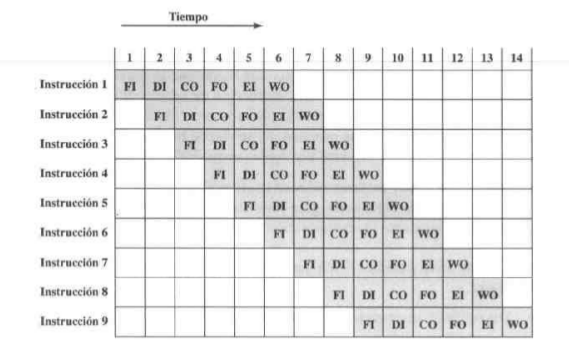
\includegraphics[scale=0.3]{imagenes/segmentacion.png} 
	\end{figure}		 		
\end{frame}

\begin{frame}
	\frametitle{Segmentación}
	\begin{block}{Conceptos}
	Sin embargo, existen problemas cuando se presentan saltos (llamado a subrutina). Como se puede observar en la siguiente figura, donde existe un salto en la instrucción 3 a la instrucción 15:
	\end{block}	
	\begin{figure}[H]
		\centering
		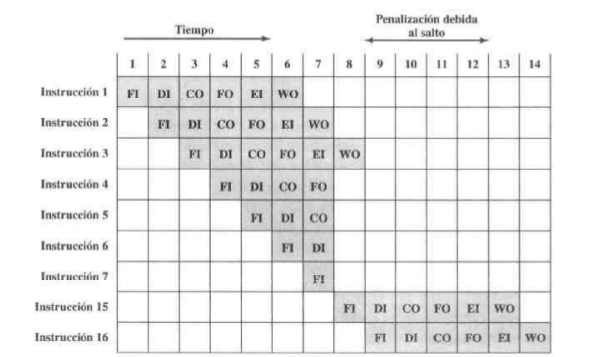
\includegraphics[scale=0.3]{imagenes/segmentacionsalto.png} 
	\end{figure}		 		
\end{frame}

\begin{frame}
	\frametitle{Segmentación}
	\begin{block}{Conceptos}
	Para enfrentar los problemas relacionados con los saltos, se diseñan estrategias para asegurar el flujo estable de las instrucciones, entre las cuales se encuentran:
	\begin{enumerate}
		\item Flujos múltiples
		\item Precaptar el salto
		\item Buffer de bucles
		\item Predicción de saltos
		\item Salto retardado
	\end{enumerate}
	\end{block}		 		
\end{frame}

\begin{frame}
	\frametitle{Segmentación}
	\begin{block}{Flujos múltiples}
	En esta estrategia se intenta resolver el problema de que cuando hay un salto, se debe escoger alguna de las dos instrucciones y se puede hacer una elección equivocada, una solución es duplicar el proceso y hacer que se ejecuten las dos instrucciones en todos los caminos posibles. El problema que se presenta retardos por el proceso adicional que se realiza.
	\end{block}		 		
\end{frame}

\begin{frame}
	\frametitle{Segmentación}
	\begin{block}{Precaptar el salto}
	Cuando se identifica un salto, se precapta la instrucción destino del salto y la siguiente despues del salto, se almacena esta ultima y se ejecuta en el momento en que se ha finalizado el salto.
	\end{block}		 		
\end{frame}

\begin{frame}
	\frametitle{Segmentación}
	\begin{block}{Buffer de bucles}
	Se almacenan las $n$ instrucciones captadas anteriormente.
	\end{block}		 		
\end{frame}

\begin{frame}
	\frametitle{Segmentación}
	\begin{block}{Predicción de saltos}
	Es intentar predecir si un salto se va a producir
	\begin{enumerate}
		\item Predecir que nunca se salta
		\item Predecir que siempre se salta
		\item Predecir según código de operación
		\item Conmutador saltar/no saltar
		\item Tabla de historia de saltos
	\end{enumerate}
	\end{block}		 		
\end{frame}

\begin{frame}
	\frametitle{Segmentación}
	\begin{block}{Salto retardado}
	Se reordenan las instrucciones de tal forma, los saltos se presenten después del momento deseado.
	\end{block}		 		
\end{frame}

\section{Paralelismo}

\begin{frame}
	\frametitle{Paralelismo}
	\begin{block}{Superescalar vs supersegmentado}
	\begin{itemize}
		\item Un procesador superescalar utiliza múltiples causes de instrucciones
		\item Un procesador supersegmentado, aprovecha que algunas etapas de las instrucciones requieren poco tiempo de realización, por lo que dobla la velocidad de procesamiento
	\end{itemize}
	\end{block}		 		
\end{frame}


\begin{frame}
	\frametitle{Paralelismo}
	\begin{block}{Superescalar vs supersegmentado}
	En la siguiente figura se puede observar la diferencia entre superescalar y supersegmentado:
	\end{block}	
	\begin{figure}[H]
		\centering
		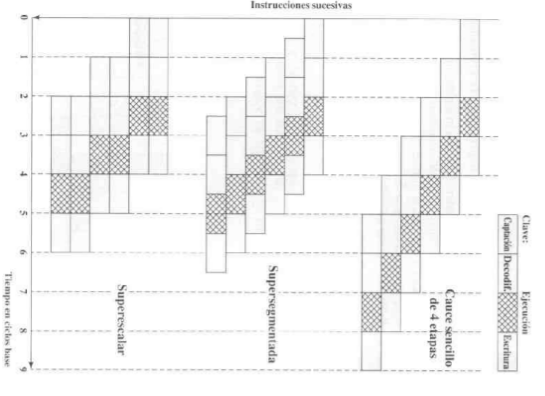
\includegraphics[scale=0.4]{imagenes/supersegmentado.png} 
	\end{figure}	 		
\end{frame}

\begin{frame}
	\frametitle{Paralelismo}
	\begin{block}{Limitaciones superescalar}
	\begin{itemize}
		\item Dependencia de datos
		\item Conflicto recursos
		\item Dependencia en salidas
	\end{itemize}
	\end{block}		 		
\end{frame}

\begin{frame}
	\frametitle{Paralelismo}
	\begin{block}{Consideraciones de diseño}
	\begin{itemize}
		\item Existe paralelismo cuando las instrucciones son independientes
		\item El paralelismo en la máquina es una medida de capacidad del procesador de sacar partido de las instrucciones
	\end{itemize}
	\end{block}		 		
\end{frame}

\begin{frame}
	\frametitle{Paralelismo}
	\begin{block}{Politicas de emisión de instrucciones}
	Para realizar el diseño de póliticas de emisión de instrucciones se tienen en cuenta las siguientes ordenaciones:
	\begin{itemize}
		\item Orden en que se captan las instrucciones
		\item Orden en que se ejecutan las instrucciones
		\item El orden en que las instrucciones actualizan registros y la memoria
	\end{itemize}
	\end{block}		 		
\end{frame}

\begin{frame}
	\frametitle{Paralelismo}
	\begin{block}{Politicas de emisión de instrucciones}
	En base a lo anterior se crean las siguientes politicas de instrucciones
	\begin{itemize}
		\item \textbf{Emisión en orden y finalización en orden:} Se ejecutan las instrucciones en el orden exacto de llegada
		\item \textbf{Emisión en orden y finalización desordenada:} Se toma en cuenta la dependencia entre salidas, por ejemplo que un recurso sea requerido por una instrucción y otra lo solicite, esta debe esperar a que el recurso esté disponible
		\item \textbf{Emisión desordenada y finalización desordenada:} Con la emisión en orden sólo de codifica hasta que exista un punto de conflicto, en este caso se siguen codificando instrucciones y ejecutando.
	\end{itemize}
	\end{block}		 		
\end{frame}

\begin{frame}
	\frametitle{Paralelismo}
	\begin{block}{Renombramiento de registros}
	Debido a la emisión y finalización desordenada de instrucciones. Debido a que pueden existir conflictos una estrategia de solución es la duplicación de recursos, la técnica es conocida como \textbf{renombramiento de registros}. Consiste en que se asigna dinámicamente los registros a las instrucciones en diversos momentos de tiempo, con esto se evita problemas en el uso de estos recursos.
	\end{block}		 		
\end{frame}

\begin{frame}
	\frametitle{Paralelismo}
	\begin{block}{Predicción de saltos}
	Debido a la segmentación de las instrucciones, existen problemas en el cause de las instrucciones debido a los saltos, en procesador superescalares la estrategia utilizada es \textbf{salto retardado}
	\end{block}		 		
\end{frame}


\begin{frame}
	\frametitle{Paralelismo}
	\begin{block}{Ejecución superescalar}
	Primero se debe analizar la dependencia entre instrucciones para enviarlas a una ventana de ejecución. Cuando se ingresan a esta ventana estas dependencias no son secuenciales (no se ejecutan en el orden de llegada), y son ejecutadas de acuerdo a la pólitica de ejecución que se utilice.
	\end{block}		 		
\end{frame}


\begin{frame}
	\frametitle{Preguntas}
	\vfill
	\begin{center}
	¿Preguntas?\\
	\vfill
	Siguiente tema: \\
	Unidad de control
	\end{center}
\end{frame}


\end{document}